\documentclass[12pt]{article}
\usepackage[pdfborder={0 0 0.5 [3 2]}]{hyperref}%
\usepackage[left=1in,right=1in,top=1in,bottom=1in]{geometry}%
\usepackage[shortalphabetic]{amsrefs}%
\usepackage{amsmath}
\usepackage{enumerate}
\usepackage{enumitem}
\usepackage{amssymb}                              
\usepackage{amsfonts}
\usepackage{amsthm}
\usepackage{bbm}
\usepackage[table,xcdraw]{xcolor}
\usepackage{tikz}
\usepackage{float}
\usepackage{booktabs}
\usepackage{svg}
\usepackage{mathtools}
\usepackage{cool}
\usepackage{url}
\usepackage{graphicx,epsfig}
\usepackage{framed}
\usepackage{hyperref}  

\usetikzlibrary{automata,arrows,positioning,calc}
\DeclarePairedDelimiter\abs{\lvert}{\rvert}%
\DeclarePairedDelimiter\norm{\lVert}{\rVert}%
\DeclarePairedDelimiter\ceil{\lceil}{\rceil}
\DeclarePairedDelimiter\floor{\lfloor}{\rfloor}

\makeatletter
\renewcommand*\env@matrix[1][*\c@MaxMatrixCols c]{%
  \hskip -\arraycolsep
  \let\@ifnextchar\new@ifnextchar
  \array{#1}}
\makeatother

\newtheorem{theorem}{Theorem}[section]
\newtheorem{corollary}{Corollary}[theorem]
\newtheorem{proposition}[theorem]{Proposition}
\newtheorem{lemma}[theorem]{Lemma}

\theoremstyle{definition}
\newtheorem{definition}[theorem]{Definition}
\newtheorem{exercise}{Exercise}%
\newtheorem{problem}[exercise]{Problem}%
\newtheorem*{example}{Example}

\theoremstyle{remark}
\newtheorem*{question}{Question}
\newtheorem*{observation}{Observation}
\newtheorem*{remark}{Remark}

\graphicspath{ {images/} }

\setlength{\parindent}{0cm}
\renewcommand{\vec}[1]{\ensuremath{\mathbf{#1}}}

\def\noi{\noindent}
\def\T{{\mathbb T}}
\def\R{{\mathbb R}}
\def\N{{\mathbb N}}
\def\C{{\mathbb C}}
\def\Z{{\mathbb Z}}
\def\P{{\mathbb P}}
\def\E{{\mathbb E}}
\def\Q{\mathbb{Q}}
\def\ind{{\mathbb I}}

\def\cale{{\mathcal E}}
\def\cals{{\mathcal S}}
\def\calc{{\mathcal C}}
\def\caln{{\mathcal N}}
\def\calb{{\mathcal B}}
\def\calg{{\cal G}}

\def\ds{\displaystyle}
\def\ra{\rightarrow}
\newcommand{\conv}{\mbox{\rm conv}}
\newcommand{\spaan}{\mbox{\rm span}}
\newcommand{\deet}{\mbox{\rm det}}
\newcommand{\aff}{\mbox{\rm aff}}
\newcommand{\cl}{\mbox{\rm cl}}
\newcommand{\dimm}{\mbox{\rm dim}}
\newcommand{\sm}{\setminus}
\def\ci{\perp\!\!\!\perp}

\newcommand{\ink}{\rule{.5\baselineskip}{.55\baselineskip}}

\begin{document}

\setcounter{section}{6}
\section{Hypothesis Testing}

\subsection{Introduction}
Statistical hypothesis testing is a formal procedure for conducting scientific inquiry according to the scientific method. In the scientific method, a scientist poses a hypothesis based on observations from nature. She then conducts an experiment to test that hypothesis, and the results of that experiment either support or refute the hypothesis. From our mathematical standpoint, a \emph{hypothesis} is a claim about one or more parameters of a population (or more than one population) of interest. For example, we might claim that a parameter equals a certain value or falls within a certain range. We then take a sample from our population and use an appropriate estimator to estimate the parameter of interest. We then use statistical techniques to either support or refute our hypotheses, and to determine the probability that we made the correct decision. \\

Here are two examples of hypothesis tests.
\begin{enumerate}
\item You are a pollster for a major news outlet, and are interested in the preferences of urban vs. rural voters in Rhode Island. Your hypothesis is that rural voters are less likely to prefer Gina Raimondo. The parameter of interest is $p_1 - p_2$, the difference in the proportion of Raimondo supporters in the two populations. You then sample registered voters from both populations and construct the estimator $\hat{p}_1 - \hat{p}_2$. Using statistics, you will be able quantify the probability that you correctly accept or reject your hypothesis based on the value of the estimator. In particular, you will be able to determine the probability that you made the \emph{wrong} decision in accepting or rejecting your hypothesis.

\item You are the principal investigator for a trial of a new drug to treat hypertension (high blood pressure). You claim that your new drug will reduce systolic blood pressure by 10 mmHg compared to a placebo pill. The parameter of interest is $\mu_1 - \mu_2$, the difference in mean blood pressure reductions between the mythical populations of all people with hypertension who would receive the drug and all people with hypertension who would receive a placebo. Your hypothesis is that $\mu_1 - \mu_2 \geq 10$. To test this, you will do a double-blind study and randomly assign 100 patients to receive the drug and 100 patients to receive the placebo pill. You will use the estimator $\bar{Y}_1 - \bar{Y}_2$ to test your hypothesis. Using statistics, you will be able quantify the probability that you correctly accept or reject your hypothesis based on the value of the estimator.
\end{enumerate}

Hypothesis testing uses the ideas we learned in the previous sections -- sampling, estimators, and confidence levels -- to 

\subsection{Elements of a Hypothesis Test}
There are four elements of any hypothesis test. We will go through an example as we discuss them. 

\begin{example}Suppose we are interested in the voting preference in Rhode Island for the gubernatorial election. 
\begin{enumerate}
\item We start with a hypothesis that we would like to support. This is called the \emph{alternative hypothesis}. For example, our alternative hypothesis could be ``More than 50\% of the voters in Rhode Island support Gina Raimondo''. In mathematical terms, our population of interest is the registered voters in Raimondo, and our parameter of interest is $p$, the proportion of registered voters who support Raimondo. The alternative hypothesis can be stated in terms of $p$ as $p > 0.5$. 
\item We will obtain support for our alternative hypothesis by showing (to a specified degree of confidence) that the \emph{null hypothesis}, the converse of the null hypothesis, is false. You may have heard of this as ``rejecting the null hypothesis''. The null hypothesis in this case is ``50\% or fewer voters in Rhode Island support Raimondo''. Mathematically, we could state this as $p \leq 0.5$ if we like. However, it turns out that this is not a useful way to state the null hypothesis. Recall that we wish to find evidence to \emph{reject} the null hypothesis. The only way to reject the hypothesis $p \leq 0.5$ is for our estimator $\hat{p}$ to produce a value over 0.5. Consider the hypothesis $p = 0.5$. Suppose our estimator $\hat{p}$ is 0.6, and we decide that this is sufficient evidence to reject the hypothesis $p = 0.5$. If we will reject $p = 0.5$, we will certainly also reject $p \leq 0.5$, since if we are willing to reject $p = 0.5$, we are even more willing to reject anything lower. Thus it suffices to take $p = 0.5$ as our null hypothesis.
\item A \emph{test statistic} is something we can actually measure which we will use to either reject or not reject the null hypothesis. In general, the test statistic will be one of our common estimators, such as $\bar{Y}$ or $\hat{p}$, or the equivalent estimators for the difference between two populations. In this case, since we are interested the population proportion $p$, we will use $\hat{p} = Y/n$ for our estimator, where $Y$ is the number of people out of a sample of size $n$ who prefer Raimondo.
\item Armed with a test statistic, the only thing left is to decide when we will reject the null hypothesis. A \emph{rejection region} (RR) specifies the values of the test statistic for which the null hypothesis will be rejected. The RR is given as a range a values. In this case, since we will reject the null hypothesis if $\hat{p}$ is \emph{high}, the rejection region will look like $\hat{p} \geq k$, where $k$ is a threshold we will choose. A lower value of $k$ means that we are more likely to reject the null hypothesis; in particular, we are more likely to reject the null hypothesis when it is in fact true, so we are more likely to commit a false positive error. Conversely, a higher value of $k$ means that we are less likely to reject the null hypothesis; in fact, we are more likely to fail to reject the null hypothesis when in fact the null hypothesis is false, thus we are more likely to commit a false positive error. Thus there is no idea value of $k$ for us to choose. We will discuss later how to pick a $k$ based on the amount of false positives and false negatives we are willing to accept.
\end{enumerate}
\end{example}

We can summarize the elements of any hypothesis test in the following table. Although the null hypothesis is ``more fundamental'', I list the alternative hypothesis first, since that lets us find the form of the null hypothesis.

\begin{framed}
\emph{Elements of a Hypothesis Test}\\
  \rule{\dimexpr\linewidth-2\fboxsep-2\fboxrule}{.1pt} \\
\begin{enumerate}
\item Alternative hypothesis, $H_a$
\item Null hypothesis, $H_0$
\item Test statistic
\item Rejection region (RR)
\end{enumerate}
\end{framed}

Before we go any further, we will take several real-world examples of hypothesis tests, and specify their four parameters. We will discuss how to choose rejection regions and how to quantify our confidence in rejecting the null hypothesis in the next sections. For completeness, the first one will be the example we did above. We will use these examples throughout this section.

\begin{enumerate}
\item You are a pollster who is interested in the voting preference in Rhode Island for the gubernatorial election. The population of interest is the number of registered voters in Rhode Island, and the parameter of interest is the $p$, the proportion of voters who are Gina Raimondo supporters.
\begin{enumerate}
\item Alternative hypothesis, $H_a: p > 0.5$
\item Null hypothesis, $H_0: p = 0.5$
\item Test statistic, $\hat{p} = Y / n$
\item Rejection region (RR), $\{\hat{p} > k\}$
\end{enumerate}

\item You are the principal investigator for a trial of a new drug to treat hypertension. The populations of interest are all patients with hypertension who receive you drug and all patients with hypertension who receive a placebo. The parameter is interest is the difference in mean blood pressure reduction $\mu_1 - \mu_2$ between these two populations.
\begin{enumerate}
\item Alternative hypothesis, $H_a: \mu_1 - \mu_2 > 10$
\item Null, $H_0: \mu_1 - \mu_2 = 10$
\item Test statistic, $\bar{Y}_1 - \bar{Y}_2$
\item Rejection region (RR), $\{\bar{Y}_1 - \bar{Y}_2 > k\}$
\end{enumerate}

\item You are a mechanical engineer and have designed a ball bearing machine which produces ball bearings which are 5 mm in diameter. Since your customers demand precision, the machine needs to be recalibrated if the average ball bearing diameter deviates from 5 mm by more than 1 percent. You suspect there might be something wrong with the machine. The population of interest is all ball bearings produces by your machine. The parameter of interest is $\mu$, the average ball bearing diameter.
\begin{enumerate}
\item Alternative hypothesis, $H_a: \mu \neq 5$
\item Null hypothesis, $H_0: \mu = 5$
\item Test statistic, $\bar{Y}$
\item Rejection region (RR), $|\bar{Y} - 5| > k$
\end{enumerate}

\end{enumerate}

Note that there is something unusual about the third example. For the first two examples, the alternative hypothesis was that the parameter of interest is \emph{above} a certain value. These are known as upper-tail hypothesis tests, since we will reject the null hypothesis if the test statistic falls in the upper tail of the appropriate probability distribution. Similarly, we could have a lower-tail hypothesis test if the alternative hypothesis is that the parameter of interest is \emph{below} a certain value. In this case, the null hypothesis would be rejected if the test statistic falls in the lower tail of the appropriate probability distribution.\\

The final example is known as a \emph{two-tailed hypothesis test}. The alternative hypothesis is that the parameter of interest is not equal to some value, i.e. that it is either above or below that value. The null hypothesis, as always, is that the parameter of interest is equal to a specific value (in this case, we do not require an additional argument to show that this makes sense).
The rejection region is stated as $|\bar{Y} - 5| > k$, indicating that we will reject the null hypothesis if the test statistic deviates from a specific value by more than a certain amount.\\

We will first discuss hypothesis tests where the sample we take is large, then we will consider the case where the sample is small. Before we do that, we will define the two types of error which can result from a hypothesis test.

\begin{framed}
\emph{Types of Error}\\
  \rule{\dimexpr\linewidth-2\fboxsep-2\fboxrule}{.1pt} \\
\begin{enumerate}
\item A \emph{type I error} is made if the null hypothesis is rejected when in fact the null hypothesis is true. The probability of making a type I error is denoted by $\alpha$:
\begin{align*}
\alpha &= \mathbb{P}(\mbox{reject null hypothesis when null hypothesis is true})\\
&= \mathbb{P}(\mbox{test statistic lies in rejection region  when null hypothesis is true})
\end{align*}

\item A \emph{type II error} is made if the null hypothesis is accepted when the alternative hypothesis is true. The probability of making a type II error is denoted by $\beta$:
\begin{align*}
\beta &= \mathbb{P}(\mbox{accept null hypothesis when alternative hypothesis is true})\\
&= \mathbb{P}(\mbox{test statistic lies outside rejection region when alternative hypothesis is true})
\end{align*}
\end{enumerate}
\end{framed}
 
Some statisticians (especially biostatisticians) will use the term \emph{power}, which is defined as $1 - \beta$.

\subsection{Large Sample Hypothesis Tests}
In this section, we will test hypotheses about the mean $\mu$ or proportion $p$ of a population. This includes the cases where we are interested in the difference between two populations. We will take a large enough sample that we can assume (by the central limit theorem) that the test statistic is normally distributed. Thus we can use the $Z$ distribution (standard normal) in our computations. \\

Let's look at one-tailed hypothesis tests first. We will do an upper-tailed test, but this is similar for lower-tailed tests. Suppose we have a parameter of interest $\theta$ (e.g. $\mu$, $p$, or the equivalent for the difference of two populations). We wish to test the alternative hypothesis $\theta > \theta_0$ (upper-tailed test), so the null hypothesis is $\theta = \theta_0$. The test statistic is the estimator $\hat{\theta}$, where we choose the appropriate estimator based on the parameter of interest. Since this is an upper-tail test, the rejection region will be of the form $\hat{\theta} > k$, where $k$ will be chosen later. Thus the parameters for the test are:

\begin{enumerate}
\item Alternative hypothesis, $H_a: \theta > \theta_0$
\item Null hypothesis, $H_0: \theta = \theta_0$
\item Test statistic, $\hat{\theta}$
\item Rejection region (RR), $\hat{\theta} > k$
\end{enumerate}

To determine the parameter $k$ in the rejection region, we fix the level $\alpha$ of type I error which we are willing to accept. If the null hypothesis is true, then the estimator $\hat{\theta}$ has a normal distribution with mean $\theta_0$ and standard deviation $\sigma_{\hat{theta}}$. Since $\alpha$ is the probability of incorrectly rejecting the null hypothesis when it is in fact true, we want to choose the rejection region such that the probability that $\hat{\theta} \geq k$ to be $\alpha$. Converting to the standard normal random variable, we want:
\begin{align*}
\P(\hat{\theta} \geq k) &= \alpha \\
\P\left( \frac{ \hat{\theta} - \theta_0 }{ \sigma_{\hat{\theta}} } \geq \frac{ k - \theta_0}{\sigma_{\hat{\theta}} }\right) &= \alpha \\
\P\left( Z \geq \frac{ k - \theta_0}{\sigma_{\hat{\theta}}} \right) &= \alpha
\end{align*}
Looking at the $Z$ table, we choose $z_\alpha$ such that $\P(Z \geq z_\alpha) = \alpha$. (On our $Z$ table, this is equivalent to $\P(Z \leq -z_\alpha) = \alpha$). Thus we have:
\begin{align*}
\frac{ k - \theta_0}{\sigma_{\hat{\theta}}}  &= z_\alpha \\
k &= \theta_0 + z_\alpha \sigma_{\hat{\theta}}
\end{align*}
This is shown in the diagram below:

\begin{figure}[H]
\centering
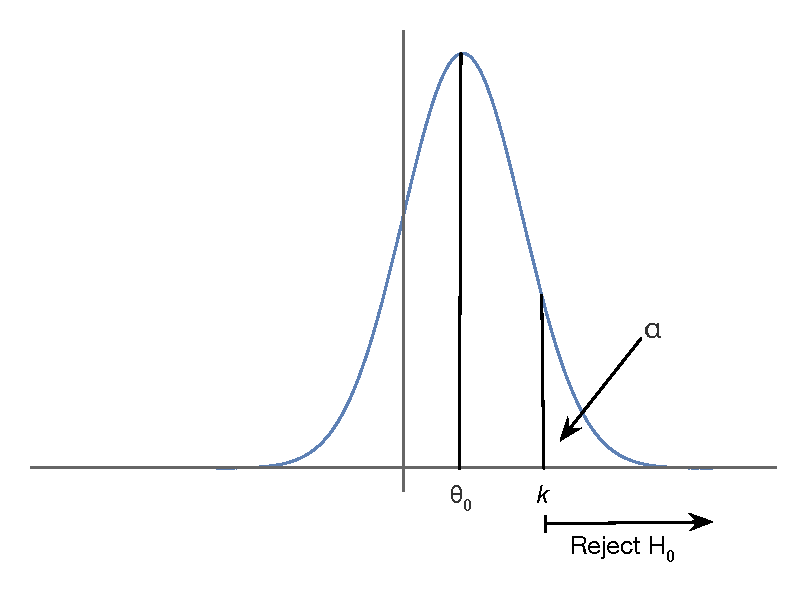
\includegraphics[width=8cm]{uppertail}
\end{figure}


Recall that $\sigma_{\hat{\theta}}$ is the standard deviation of the estimator, which is computed from the the population standard deviation and the sample size. If we do not know the population standard deviation, we can use the sample standard deviation $S$ in place of the population standard deviation $\sigma$ since the sample size is large.

\begin{example}
You are a pollster who is interested in the voting preference in Rhode Island for the gubernatorial election. The population of interest is the number of registered voters in Rhode Island, and the parameter of interest is the $p$, the proportion of voters who support Gina Raimondo. Suppose you sample 100 voters and 60 of them favor Raimondo. Does the evidence support Raimondo being favored at a level of 0.05?\\

The parameters of the test are given above. The test statistic is $\hat{p} = 0.6$. To find the appropriate rejection region at a level of $\alpha = 0.05$ we need to find the appropriate value of $z_\alpha$ from the $Z$ table. Looking at the table, we find that $z_\alpha = 1.64$ (we could also have chosen 1.65). We do not know the population standard deviation, but we can estimate it by using $\hat{p}$ in place of the true value $p$:
\[
\sigma_{\hat{\theta}} = \sqrt{ \frac{p(1-p)}{n} } \approx \sqrt{ \frac{\hat{p}(1-\hat{p})}{n} } = \sqrt{ \frac{(0.6)(0.4)}{100}} = 0.049
\] 
From this we calculate:
\[
k = 0.5 + z_\alpha \sigma_{\hat{\theta}} = 0.5 + 1.64 (0.049) = 0.58
\]
Thus the rejection region is
\[
\{ \hat{p} \geq 0.58 \}
\]
Since our test statistic is 0.6, it falls inside the rejection region, thus we can reject our null hypothesis with a level of 0.05, so we are 95\% confident that Raimondo is favored in the population at large.
\end{example}

Similarly, we can do this for a two-tailed hypothesis test. Here we ``split'' the $\alpha$ between the upper and lower tails of the normal distribution.
\begin{align*}
\P(|\hat{\theta} - \theta_0 | \geq k) &= \alpha \\
\P\left(\left|\frac{ \hat{\theta} - \theta_0 }{ \sigma_{\hat{\theta}} } \right| \geq \frac{k}{\sigma_{\hat{\theta}}} \right) &= \alpha \\
\P\left( |Z| \geq \frac{k}{\sigma_{\hat{\theta}}} \right) &= \alpha \\
\end{align*}
Splitting the $\alpha$ evenly between the upper and lower tails, we want
\[
\P\left(Z \leq -\frac{k}{\sigma_{\hat{\theta}}} \right) = \alpha / 2
\]
and
\[
\P\left(Z \geq \frac{k}{\sigma_{\hat{\theta}}} \right) = \alpha / 2
\]
In the same way as before, we can use the $Z$ table to find the appropriate value of $z_{\alpha/2}$. Thus we have:
\begin{align*}
\frac{k}{\sigma_{\hat{\theta}}} &= z_{\alpha/2}\\
k &= z_{\alpha/2} \sigma_{\hat{\theta}}
\end{align*}
Our rejection region is:
\[
\{ |\hat{\theta} - \theta_0| \geq  z_{\alpha/2} \sigma_{\hat{\theta}} \}
\]
The diagram below shows the rejection region for a two-tailed test in terms of the standard normal $Z$ distribution.

\begin{figure}[H]
\centering
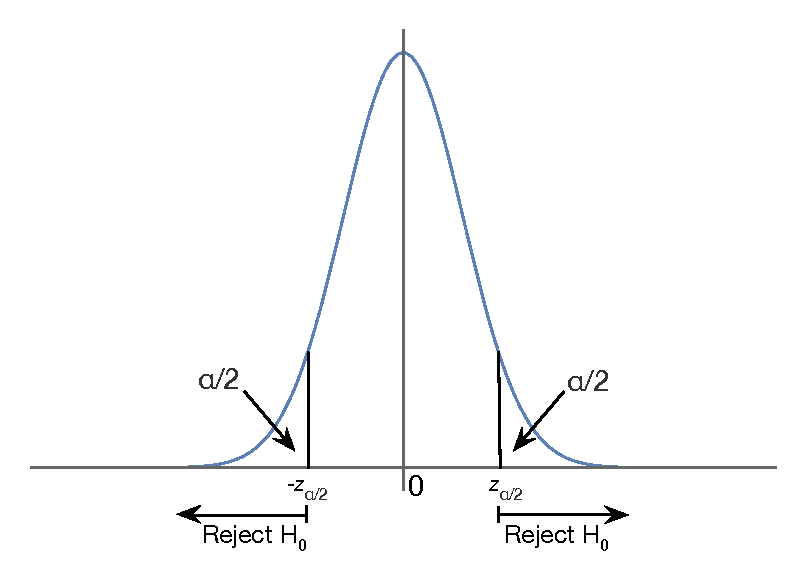
\includegraphics[width=8cm]{twotailed}
\end{figure}

Let's do our ball bearing example.

\begin{example}You are a mechanical engineer and have designed a ball bearing machine which produces ball bearings which are 5 mm in diameter. You suspect there might be something wrong with the machine. You sample 64 ball bearings from the machine, and obtain a sample mean of 4.98 mm and a sample standard deviation of 0.1 mm. Can you conclude at a level of 0.95 that there is something wrong with the machine?

The parameters of the test are given above. The test statistic is $\bar{Y} = 4.98$. To find the appropriate rejection region at a level of $\alpha = 0.05$, since this is a two-sided hypothesis test, we need to find the appropriate value of $z_{\alpha/2}$ from the $Z$ table. Looking at the table, we find that $z_\alpha = 1.96$. We do not know the population standard deviation, but we can estimate it by using $S$ in place of $\sigma$. The standard deviation of the estimator is therefore approximately:
\[
\sigma_{\bar{Y}} \approx \frac{S}{\sqrt{n}} = \frac{0.1}{\sqrt{64}} = \frac{0.1}{8} = 0.0125
\]
Thus our value of $k$ is:
\[
k = z_{\alpha/2} \sigma_{\bar{Y}} = 1.96 (0.0125) = 0.0245
\]
The rejection region is therefore:
\[
\{ |\bar{Y} - 5 | \geq 0.0245 \} = \{ \bar{Y} \leq 4.9755 \text{ or } \bar{Y} \geq 5.0245 \}
\]
Since out test statistic does not fall within our rejection region, we do not reject the null hypothesis, so for now you conclude that you do not have to do maintenance on the machine.
\end{example}

\subsection{Large Sample Hypothesis Tests and Type II Error}
We have discussed how to choose the rejection region based on the level of type I error we are willing to accept. Now we will discuss type II error. We will only quantify type II error for one-tailed hypothesis tests. For two-tailed tests, this process is arduous, thus will be omitted. The discussion below will concern upper-tail hypothesis tests. Lower-tail tests are similar, except everything is ``flipped''.\\

Recall that a type II error is made if we accept the null hypothesis when in fact the null hypothesis is false. In other words, our test statistic falls \emph{outside} the rejection region, even though the null hypothesis is false and should be rejected. When evaluating type II error, we need to make an additional decision. We need to specify a \emph{specific} value of the alternative hypothesis to be a \emph{positive test threshold} (my own term) which we will use to compute $\beta$.\\

Let's use the same upper-tail setup as before. Suppose we have a parameter of interest $\theta$. We wish to test the alternative hypothesis $\theta > \theta_0$ (upper-tailed test), so the null hypothesis is $\theta = \theta_0$. The test statistic is the estimator $\hat{\theta}$, and the rejection region is of the form $\{\hat{\theta} > k\}$. For now, assume we have chosen $k$ according to our desired $\alpha$ using the methods of the previous section. To reiterate, our test has the following parameters:

\begin{enumerate}
\item Alternative hypothesis, $H_a: \theta > \theta_0$
\item Null hypothesis, $H_0: \theta = \theta_0$
\item Test statistic, $\hat{\theta}$
\item Rejection region (RR), $\{ \hat{\theta} > k \}$
\end{enumerate}

We will choose a specific value $\theta_a$ for the alternative hypothesis (our positive test threshold). Since this is an upper tail test, we must have $\theta_a > \theta_0$. Then $\beta$, the probability of a type II error, is defined as the probability of accepting the null hypothesis when the true value of the parameter is in fact $\theta_a$.\\

It seems odd that we must specify a value for $\theta_a$ in order to do this, but this has a nice interpretation. The probability of accepting the null hypothesis if the true parameter is $\theta_a$ is $\beta$. If the true value of $\theta$ is greater than $\theta_a$, the probability of accepting the null hypothesis is less than $\beta$. Thus if the true value of $\theta$ is $\theta_a$ or greater, the probability that we will incorrectly accept the null hypothesis is at most $\beta$.\\

Now that we've gotten that out of the way, how we we actually find $\beta$? Take a look a the following picture:

\begin{figure}[H]
\centering
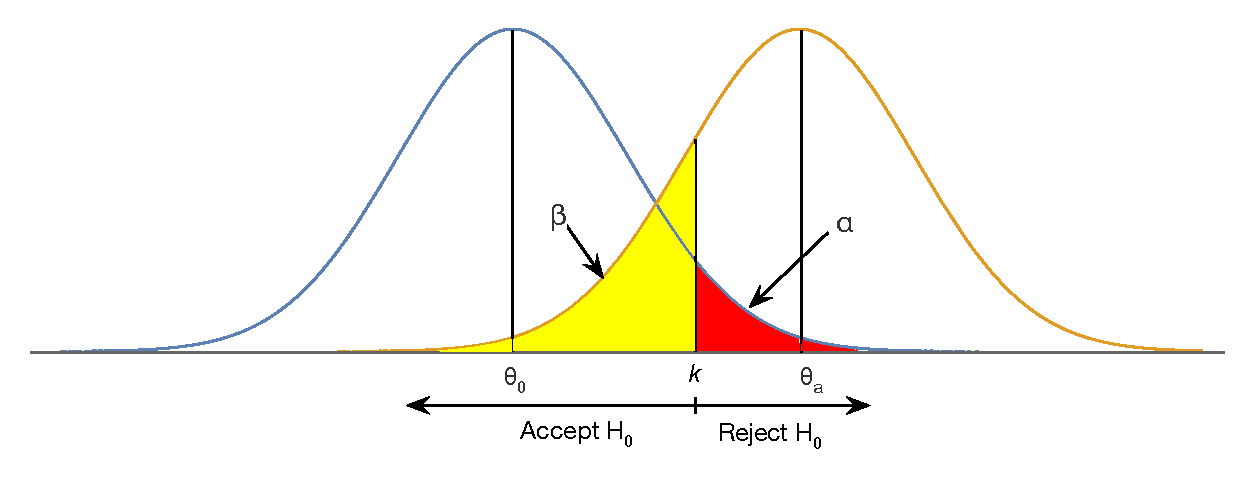
\includegraphics[width=12cm]{alphabeta}
\end{figure}

$\beta$ is the probability that the test statistic lies outside the rejection region when the true value of the parameter is $\theta_a$. This time, the estimator has a normal distribution with mean $\theta_a$ and standard deviation $\sigma_{\hat{\theta}}$. Thus, for the upper tail test here, we want the probability that our test statistic is less than $k$, the threshold of the rejection region.

\begin{align*}
\beta &= \P(\hat{\theta} \leq k)\\
&= \P\left( \frac{ \hat{\theta} - \theta_a }{ \sigma_{\hat{\theta}} } \leq \frac{ k - \theta_a}{\sigma_{\hat{\theta}} }\right) \\
&= \P\left( Z \leq \frac{ k - \theta_a}{\sigma_{\hat{\theta}}} \right)
\end{align*}
Since we know $\theta_a$ and $\sigma_{\hat{\theta}}$, and since we have already computed the boundary of the rejection region $k$, we can use the $Z$ table to solve for $k$

Let's go back and do our polling example from above.

\begin{example}
You are again a pollster who is interested in the voting preference in Rhode Island for the gubernatorial election. The population of interest is the number of registered voters in Rhode Island, and the parameter of interest is the $p$, the proportion of voters who are Gina Raimondo supporters. You sample 100 voters and 60 of them favor Raimondo. You create a hypothesis test with $\alpha = 0.05$, for which we have seen that the rejection region is $\{ \hat{p} \geq 0.58 \}$. For a value of the alternative hypothesis $p_a = 0.60$, calculate $\beta$, the probability of a type II error.\\

Given our discussion above, plugging in the values we determined in the example above ($k = 0.58$, $\sigma_{\hat{\theta}} = 0.049$), and using $p_a = 0.60$:
\begin{align*}
\beta &= \P\left( Z \leq \frac{ k - p_a}{\sigma_{\hat{p}}} \right) \\
&= \P\left( Z \leq \frac{ 0.58 - 0.60}{ 0.049 } \right) \\
&= \P (Z \leq -0.41 )\\
&= 0.3409
\end{align*}
\end{example}

\subsection{Sample Size Selection}

If you are a scientist devising a hypothesis test, you don't want to just run the test and calculate $\beta$ after the fact the way we did in the example above. If you did that, $\beta$ might be too large, and your test could be meaningless! You would like a procedure where, if you specify the maximum values of $\alpha$ and $\beta$ you are willing to tolerate, you can compute the size of the sample $n$ you need to attain these values. Along the way, you will also compute $k$, the threshold for the rejection region. The following derivation is for an upper-tail hypothesis test. A similar derivation will work for a lower-tail test. The two-tailed test will not be discussed.\\

For simplicity, we will do the computation for a hypothesis test involving the sample mean. We can similarly do this for a hypothesis test involving the sample proportion. As an experimenter, you are conducting an upper tail hypothesis test with the following four parameters:
\begin{enumerate}
\item Alternative hypothesis, $H_a: \mu > \mu_0$
\item Null hypothesis, $H_0: \mu = \mu_0$
\item Test statistic, $\bar{Y}$
\item Rejection region (RR), $\{ \bar{Y} > k \}$
\end{enumerate}
In addition, you need to choose three more parameters:
\begin{enumerate}
\item $\theta_a$, a specific value of the alternative hypothesis. As before, we require $\theta_a > \theta_0$
\item $\alpha$, the maximum type I error you are willing to accept
\item $\beta$, the maximum type II error you are willing to accept
\end{enumerate}
The population standard deviation is denoted $\sigma$. If we do not know $\sigma$, we can estimate it by the sample standard deviation $S$. In the real world, to obtain $S$, we can do a pilot study for the express purposes of computing $S$. We just need to make sure that the pilot study is large enough that the $S$ we obtain is a good estimator for $\sigma$.\\

As above, we will write the appropriate equations for $\alpha$ and $\beta$. Since we will have two equations and only two unknowns ($k$ and $n$), we can solve them for the unknowns. Using the definition of $\alpha$ and referring to the picture above:
\begin{align*}
\alpha &= \P( \text{test statistic is in rejection region when null hypothesis is true} )\\
&= \P( \bar{Y} \geq k \text{ when } \mu = \mu_0  ) \\
&= \P\left( \frac{ \bar{Y} - \mu_0}{ \sigma / \sqrt{n} } \geq  \frac{ k - \mu_0}{ \sigma / \sqrt{n} } \right) \\
&= \P(Z \geq z_\alpha )
\end{align*}
where $z_\alpha$ is chosen from our $Z$-table so that $\P(Z \geq z_\alpha) = \alpha$. Using the definition of $\beta$ and again referring to the picture above:
\begin{align*}
\beta &= \P( \text{test statistic is outside rejection region when alternative hypothesis is true} )\\
&= \P( \bar{Y} \leq k \text{ when } \mu = \mu_a ) \\
&= \P\left( \frac{ \bar{Y} - \mu_a}{ \sigma / \sqrt{n} } \leq  \frac{ k - \mu_a}{ \sigma / \sqrt{n} } \right) \\
&= \P(Z \leq -z_\beta )
\end{align*}
where $z_\beta$ is chosen from our $Z$-table so that $\P(Z \leq -z_\beta) = \beta$. We use the negative sign for convenience, since the value of $z$ we are looking for will always fall to the left of 0 on a graph of the standard normal distribution. We then have two equations we can solve simultaneously:
\begin{align*}
\frac{ k - \mu_0}{ \sigma / \sqrt{n} } &= z_\alpha \\
\frac{ k - \mu_a}{ \sigma / \sqrt{n} } &= -z_\beta
\end{align*}
If we solve both equations for $k$, we get:
\begin{align*}
k &= \mu_0 + z_\alpha \frac{\sigma}{\sqrt{n}} \\
k &= \mu_a - z_\beta \frac{\sigma}{\sqrt{n}} 
\end{align*}
We can use the first equation in the set above to find $k$, the boundary of the rejection region. This is the same equation we derived in the section on large sample hypothesis tests. Setting these two equations equal to each other:
\begin{align*}
\mu_0 + z_\alpha \frac{\sigma}{\sqrt{n}} &= \mu_a - z_\beta \frac{\sigma}{\sqrt{n}} \\
(z_\alpha + z_\beta)\frac{\sigma}{\sqrt{n}} &= \mu_a - \mu_0 \\
\sqrt{n} &= \frac{(z_\alpha + z_\beta)\sigma}{\mu_a - \mu_0 }\\
n &= \frac{(z_\alpha + z_\beta)^2\sigma^2}{(\mu_a - \mu_0)^2 }
\end{align*}

\subsection{p-values}
The parameter $\alpha$ is the probability of making a type I error, i.e. rejecting the null hypothesis when it is in fact true. Generally, experimenters choose small values of $\alpha$ to maximize their confidence that a positive result is not a false positive, i.e. due to chance alone. Typical values of $\alpha$ you will see in the scientific literature are 0.05 and 0.01, although this is a little arbitrary. \\

Another way of reporting the probability of a type I error is the $p$-value. This is what is most often given in the scientific literature.

\begin{framed}
\emph{$p$-value}\\
  \rule{\dimexpr\linewidth-2\fboxsep-2\fboxrule}{.1pt} \\
The $p$-value, or attained significance level, of a test is the smallest level of significance $\alpha$ for which the test statistic indicates that the null hypothesis should be rejected.
\end{framed}

In other words, for any $\alpha$ greater than or equal to the $p$-value, the null hypothesis can be rejected using the test statistic. For $\alpha$ less than the $p$-value, the null hypothesis cannot be rejected. This provides more information than just saying that the null hypothesis was rejected for a certain value of $\alpha$. The following picture may be useful. It shows an upper-tail hypothesis test, but this can be computed for any hypothesis test. The null hypothesis is given by $\theta_0$, and the test statistic is $\hat{\theta}$.

\begin{figure}[H]
\centering
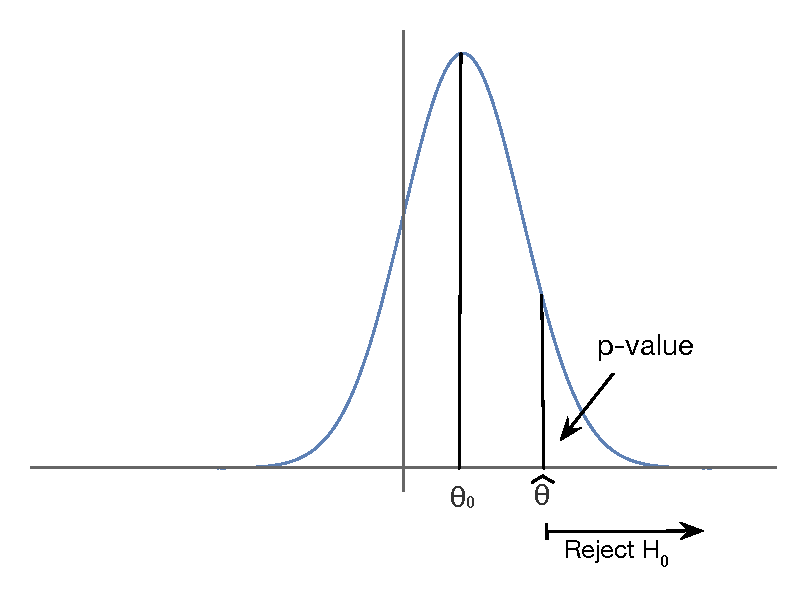
\includegraphics[width=8cm]{pvalues}
\end{figure}

Let's look at our voter polling example from before.

\begin{example}
You are a pollster who is interested in the voting preference in Rhode Island for the 2016 gubernatorial election. The population of interest is the number of registered voters in Rhode Island, and the parameter of interest is the $p$, the proportion of voters who support Gina Raimondo. Suppose you sample 100 voters and 60 of them favor Raimondo. What is the $p$-value for this test? (It is a little confusing that $p$ is the sample proportion and we also have a $p$-value for the test, but this notation is standard in both cases; we will write the $p$-value as ``$p$-value'' rather than just $p$ to avoid this confusion).\\

We want the smallest value of $\alpha$ for which we will reject the null hypothesis. The value we obtained for $\hat{p}$ is 0.6. We estimated the standard deviation of the estimator $\hat{p}$ as 0.049 above (this include the factor of $\sqrt{n}$ in the denominator). Thus we have:
\begin{align*}
p\text{-value} &= \P(\hat{p} \geq 0.6 \text{ given null hypothesis is true})\\
&= \P(\hat{p} \geq 0.6 \text{ given } p = 0.5)\\
&= \P \left( \frac{\hat{p} - 0.5}{\sigma_{\hat{p}}} \geq \frac{0.6 - 0.5}{\sigma_{\hat{p}}} \right) \\
&= \P \left( Z \geq \frac{0.1}{0.049} \right)\\
&= \P (Z \geq 2.04)\\
&= 0.0207
\end{align*}
Thus we have a $p$-value of 0.0207, which is the smallest value of $\alpha$ for which the test statistic indicates that we can reject the null hypothesis. Above, we showed that we can reject the null hypothesis with an $\alpha$ of 0.05. This is consistent with our $p$-value, since 0.05 is greater than the $p$-value.
\end{example}

\subsection{Small sample hypothesis testing for the population mean}
In the previous section, we discussed hypothesis testing procedures for large samples. The large sample assumption is important because that guarantees that the test statistic has a normal distribution (by the central limit theorem). The large sample size also allows us to estimate the population standard deviation using the sample standard deviation.\\

What happens when the sample size is not large? As in the section on confidence intervals, if we have a population that is normally distributed with unknown standard deviation, we can use the $t$-distribution in place of the $Z$ distribution. Suppose we have a normally-distributed population, and we take a small sample ($n < 30$) from that population. The population standard deviation is unknown, so we estimate it with the sample standard deviation $S$. Suppose we are are doing an upper-tailed hypothesis test. Let $\mu = \mu_0$ be the null hypothesis, and $\mu > \mu_0$ be the alternative hypothesis. The test statistic is $\bar{Y}$, the standard unbiased estimator for $\mu$. Then to find the appropriate rejection region based on our desired level $\alpha$, we follow the same procedure above except that we use the $t$ distribution with $n-1$ df in place of the $Z$ distribution. This works because
\[
T = \frac{ \bar{Y} - \mu_0}{S/\sqrt{n}}
\]
has a $t$ distribution with $n-1$ df. For example, if we are doing an upper-tail test with desired level $\alpha$, then the rejection region is given by:
\begin{align*}
k &= \mu_0 + t_\alpha \sigma_{\bar{Y}}\\
&= \mu_0 + t_\alpha \frac{S}{\sqrt{n}}
\end{align*}
All we did to get this formula was replace the $z$ with a $t$. We will return to our rocket science example from the section on confidence intervals.

\begin{example}You are a rocket scientist, and you conduct an experiment which involves measuring the launch velocity of a model rocket. You claim that the launch velocity of the model rocket is more than 29 m/s. Suppose 8 measurements are taken. The sample mean is 29.59 m/s, and the sample standard deviation is 0.391 m/s. Is the claim supported at the 0.025 level of significance?\\

This is an upper-tailed hypothesis test with the following parameters:
\begin{enumerate}
\item Alternative hypothesis, $H_a: \mu > 29$
\item Null hypothesis, $H_0: \mu = 29$
\item Test statistic, $\bar{Y}$
\item Rejection region (RR), $\{ \bar{Y} > k \}$
\end{enumerate}
We assume that the launch velocities are normally distributed (a normally distributed population is essential for use to use the $t$-distribution). For the rejection region, we have:
\begin{align*}
k &= \mu_0 + t_\alpha \sigma_{\bar{Y}} \\
&= 29 + t_\alpha \frac{S}{\sqrt{n}} \\
&= 29 + t_{0.025} \frac{0.391}{\sqrt{8}} \\
&= 29 + 2.365 ( 0.138 ) \\
&= 29.326
\end{align*}
The rejection region is $\{\bar{Y} \geq 29.326\}$. Since our measurement lies in the rejection region, we can reject the null hypothesis with a level of $0.025$. Thus the claim is supported at the 0.025 level of significance.
\end{example}

\subsection{Power of Hypothesis Tests}
In the previous sections, we have discussed large-sample and small-sample hypothesis tests for various test statistics. We learned how to specify a rejection region for a desired $\alpha$ and how to compute $\beta$ for a specific value of the alternative hypothesis. How did we decide on those test statistics, and how do we know we selected the best rejection region. In other words, how ``good'' are the tests?\\

So far, we have used the parameters $\alpha$ and $\beta$, the probabilities of type I and type II error, to measure the ``goodness'' of a hypothesis test. Recall that to compute $\beta$ we had to choose a specific value for the alternative hypothesis $\theta_a$. We would like a function which gives us the error of the test given the true value of the parameter. The function we use is called the power of a hypothesis test.

\begin{framed}
\emph{Power of a Hypothesis Test}\\
  \rule{\dimexpr\linewidth-2\fboxsep-2\fboxrule}{.1pt} \\
Suppose we have a hypothesis test, with test statistic $\hat{\theta}$ and rejection region RR. Then the \emph{power} of the hypothesis test, denoted $Power(\theta)$ is the probability that the test statistic $\hat{\theta}$ will lie in the rejection region if the true parameter value is $\theta$, i.e.
\[
Power(\theta) = \P(\hat{\theta} \text{ lies in RR when true parameter value is }\theta )
\]  
\end{framed}
The power function relates $\alpha$ and $\beta$ in the following way. Suppose our null hypothesis is $\theta_0$, and we have chosen the specific value $\theta_a$ for our alternative hypothesis. Let $\alpha$ be the probability of a type I error, and let $\beta(\theta_a)$ be the probability of a type II error when the true value is $\theta_a$. Then we observe the following:
\begin{enumerate}
\item $Power(\theta_0) = \alpha$ since $Power(\theta_0)$ is the probability of rejecting the null hypothesis when it is true.
\item $Power(\theta_a) = 1 - \beta(\theta_a)$, since $\beta(\theta_a)$ is the probability of accepting the null hypothesis when $\theta_a$ is true.
\end{enumerate}
For an ideal test, the power function would be 0 at $\theta_0$ and 1 for all possible values of the alternative hypothesis $\theta_a$. Here is what this would look like graphically for a two-tailed hypothesis test.

\begin{figure}[H]
\centering
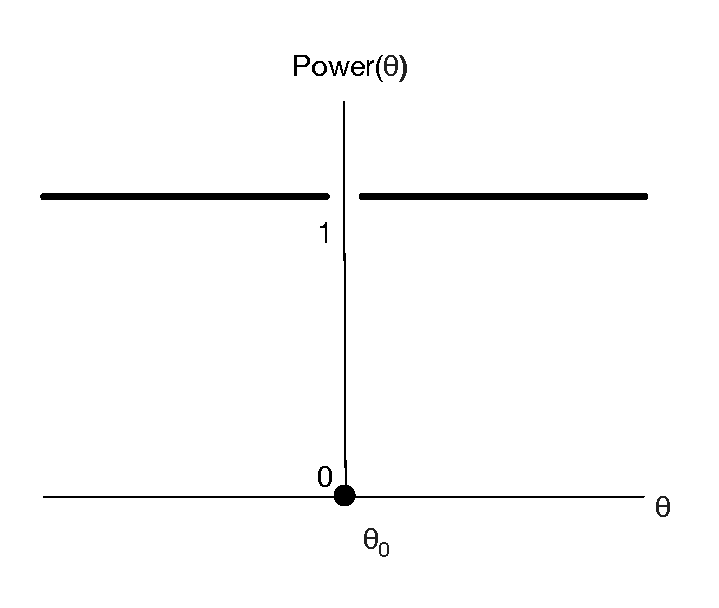
\includegraphics[width=8cm]{idealpower}
\end{figure}

No hypothesis test, however, is perfect. Realistically, the power curve for a two-tailed hypothesis test will look more like this:

\begin{figure}[H]
\centering
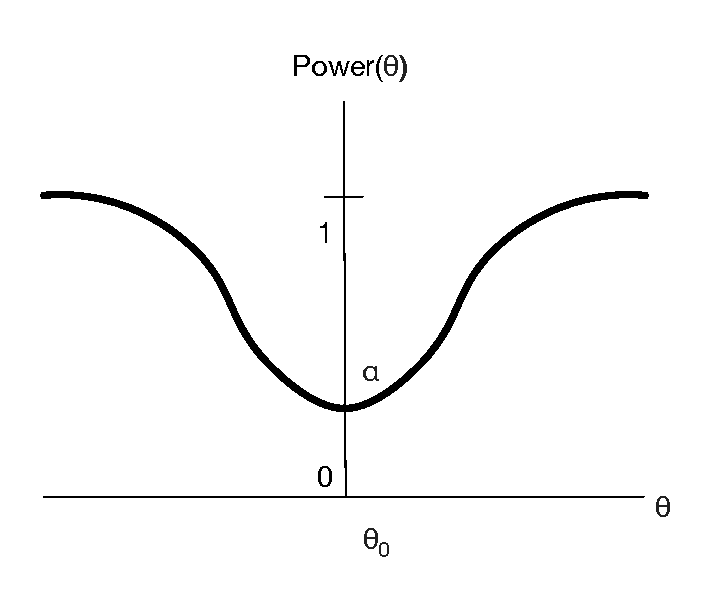
\includegraphics[width=8cm]{realpower}
\end{figure}

What we would like is a test which maximizes the power function for a given $\alpha$. This is called the \emph{most powerful $\alpha$-level test}. Before we state the condition under which we have such a test, we need one more set of definitions.

\begin{framed}
\emph{Simple and Composite Hypotheses}\\
  \rule{\dimexpr\linewidth-2\fboxsep-2\fboxrule}{.1pt} \\
Suppose we have a random sample taken from a population with parameter $\theta$, and consider a hypothesis specifying the value of $\theta$. If the hypothesis uniquely specifies the distribution of the population, we call our hypothesis a \emph{simple hypothesis}. Otherwise, we call it a \emph{composite hypothesis}.
\end{framed}
Let's look at examples of simple and composite hypotheses.
\begin{example}
\begin{enumerate}
\item Suppose we have a population which is normally distributed with mean $\mu$ and variance 1. Since the distribution of the population is uniquely specified by $\mu$, a hypothesis involving $\mu$ such as the null hypothesis $\mu_0 = 0$, is a simple hypothesis.
\item Suppose we have a population which is normally distributed with mean $\mu$ and unknown variance $\sigma^2$. Here we need both $\mu$ and $\sigma_2$ to specify the distribution of the population, so a hypothesis involving $\mu$ such as the null hypothesis $\mu_0 = 0$, is a composite hypothesis.
\item Suppose we have a population with is exponentially distributed with parameter $\lambda$. Then a hypothesis involving $\lambda$ is a simple hypothesis since $\lambda$ uniquely specifies the distribution of the population. Since the population mean $\mu = 1 / \lambda$, a hypothesis involving the mean $\mu$ is also a simple hypothesis.
\end{enumerate}
\end{example}
Consider a hypothesis test where we are testing a simple null hypothesis $\theta = \theta_0$ against a simple alternative hypothesis $\theta = \theta_a$. We would like to choose a rejection region such that:
\begin{enumerate}
\item $Power(\theta_0) = \alpha$
\item $Power(\theta_a)$ is as large as possible
\end{enumerate}
In other words, we are looking for the most powerful $\alpha$-level test. The following theorem tells us how to derive the most powerful $\alpha$-level test in this case.
\begin{framed}
\emph{Neyman-Pearson Lemma}\\
  \rule{\dimexpr\linewidth-2\fboxsep-2\fboxrule}{.1pt} \\
Suppose we have a population whose distribution parameterized by $\theta$. Suppose we have a hypothesis test in which we wish to test the simple null hypothesis $H_0: \theta = \theta_0$ against the simple alternative hypothesis $H_a: \theta = \theta_a$. We do this by taking a random sample $Y_1, \dots, Y_n$ drawn from the population. Let $L(Y_1, \dots, Y_n|\theta)$ be the likelihood function for the sample when the value of the parameter is $\theta$. Then, for a given $\alpha$, the test that maximizes the power for the alternative hypothesis $\theta_a$ has a rejection region given by:
\[
\frac{ L(Y_1, \dots, Y_n|\theta_0) }{ L(Y_1, \dots, Y_n|\theta_a)} < k
\]
where the value of $k$ is chosen so that the test has the desired $\alpha$. The ratio of likelihood functions is called a \emph{likelihood ratio}. Such a test is the most powerful $\alpha$-level test for $H_0$ versus $H_a$.
\end{framed}

Let's look at an example application of this theorem.

\begin{example}Suppose $Y$ is a single observation from a population parameterized by $\theta$ with probability density function
\[
f_\theta(y) = \begin{cases}
\theta y^{\theta - 1} & 0 < y < 1 \\
0 & \text{otherwise}
\end{cases}
\]
Find the most powerful hypothesis test with $\alpha = 0.05$ to test the null hypothesis $H_0: \theta = 2$ against the alternative hypothesis $H_a: \theta = 1$.\\

Since the distribution of the population is uniquely determined by the parameter $\theta$, both hypotheses are simple, so we can use the Neyman-Pearson lemma to derive the most powerful test. Since there is only one sample, the likelihood ratio is given by:
\[
\frac{L(Y|\theta_0)}{L(Y|\theta_a)} = \frac{f_{\theta_0(Y)}}{f_{\theta_a(Y)}} = \frac{2(Y)}{1(Y^0)} = 2Y  
\]
So the rejection region is of the form $2Y < k$, where we will determine $k$ based on the desired level $\alpha = 0.05$. Dividing by 2, we get $Y < k/2$, and letting $m = k/2$, the rejection region is of the form $Y < m$. We determine $m$ based on the definition of $\alpha$.
\begin{align*}
0.05 &= \alpha = \P(Y \text{ lies in RR when the null hypothesis is true})\\
&= \P(Y \text{ lies in RR when }\theta = 2)\\
&= \P(Y < m \text{ when }\theta = 2)\\
&= \int_0^m 2y dy\\
&= m^2
\end{align*}
Thus we have $m^2 = 0.05$, so $m = \sqrt{0.05} = 0.2236$. Thus the rejection region for the 0.05-most powerful test is:
\[
\{ Y < 0.2236 \}
\]
In other words, among all hypothesis tests for $H_0: \theta = 2$ versus $H_a: \theta = 1$ based on a sample size of 1 and $\alpha = 0.05$, this test has the largest possible value for $Power(\theta_a) = Power(1)$. Equivalently, this test has the smallest type II error given a sample size of 1 and $\alpha = 0.05$ for this specific pair of alternative and null hypotheses. What is the actual value of $Power(1)$ in this case. Using the definition of the power of a hypothesis test,
\begin{align*}
Power(1) &= \P(Y \text{ lies in RR when }\theta = 1)\\
&= \P(Y < 0.2236 \text{ when }\theta = 1)\\
&= \int_0^{0.2236} 1 dy\\
&= 0.2236
\end{align*}
The value 0.2236 is the maximum value of the power of the test among all tests with $\alpha = 0.05$. But for this test, $\beta = 1 - 0.2236 = 0.7764$, which is very large. So this test is not very good. However, no other test with these same parameters is any better.
\end{example}
What about our hypothesis tests from the previous section. It turns out that they are the uniformly best hypothesis tests for the given situations. We give one example (without proof) below.

\begin{example}
Suppose $Y_1, \dots, Y_n$ are samples drawn from a normal distribution with unknown mean $\mu$ and known variance $\sigma^2$. We wish to test the null hypothesis $H_0: \mu = \mu_0$ against the alternative hypothesis $H_a: \mu > \mu_0$. Then the $\alpha$-most powerful test is given by $\bar{Y} > k$, where
\[
k = \mu_0 + z_\alpha\frac{\sigma}{\sqrt{n}}
\]
This is the test statistic and rejection region we used earlier for large-sample hypothesis testing. Thus our large sample hypothesis test using the $Z$-distribution is in fact the best hypothesis test we can construct. The proof of this result is an application of the Neyman-Pearson lemma. It is relatively straightforward, but the calculus and algebra are messy, so we will omit that here.
\end{example}

\subsection{Likelihood Ratio Tests}
In the previous section, we learned how to construct the most powerful $\alpha$-level test for simple hypotheses. In this case, the distribution of the population is known except for the value of a single parameter $\theta$, and the null and alternative hypothesis are specified in terms of $\theta$. The Neyman-Pearson lemma shows us how to use a likelihood ratio test to construct the most powerful $\alpha$-level test.\\

In many cases, we are interested in testing hypotheses involving one parameter, but the population has more than one unknown parameter. We have already encountered this in the section on small-sample hypothesis tests for the mean of normally distributed populations where the population variance is unknown. In this case, the parameter of interest is the population $\mu$. We don't care about the unknown population standard deviation $\sigma$, so it is called a \emph{nuisance parameter}. We are also interested in cases where we do not have to choose a specific value for the alternative hypothesis, like we did when we used the Neyman-Pearson lemma. In both these cases (multiple unknown parameters and more complicated alternative hypotheses), we can use a \emph{likelihood ratio test}.\\

Here is the setup for a likelihood ratio test:
\begin{enumerate}
\item We have a population which is parameterized by a set of parameters $\Theta = (\theta_1, \dots, \theta_n)$. For example, if the population is normally distributed, it is parameterized by $\Theta = (\mu, \sigma)$.
\item We take a sample of size $n$ of independent samples $Y_1, \dots, Y_n$ from the population.
\item Given specific values of the parameters $\Theta = (\theta_1, \dots, \theta_n)$, the likelihood function for our sample is denoted $L(Y_1, \dots, Y_n|\Theta)$. For a normally distributed population, our likelihood function will depend on $\Theta = (\mu, \sigma)$.
\item The null hypothesis states that $\Theta$ lies in a particular set of values $\Omega_0$, where the alternative hypothesis states that $\Theta$ lies in another set of values $\Omega_a$, where $\Omega_0$ and $\Omega_a$ must be disjoint (it does not make sense otherwise). Note that the null and alternative hypotheses no longer need to be single points. They do not have to be simple hypotheses since they can contain unknown parameters or multiple values of a parameter. For example, if we have a population which is exponentially distributed with parameter $\lambda$, then if we want to test the null hypothesis $H_0: \lambda = \lambda_0$ versus the alternative hypothesis $\lambda \neq \lambda_0$, then we would have $\Omega_0 = \{ \lambda_0 \}$ and $\Omega_a = \{ \lambda > 0 : \lambda \neq \lambda_0 \}$.
\item The \emph{parameter space} is defined to be $\Omega = \Omega_0 \cup \Omega_a$, which is all possible values of the parameters. In the exponential example $\Omega = \{ \lambda > 0 \}$, which is all possible values of an exponential parameter.
\item We define:
\begin{align*}
L(\hat{\Omega}_0) &= \max_{\Theta \in \Omega_0} L(Y_1, \dots, Y_n|\Theta) \\
L(\hat{\Omega}) &= \max_{\Theta \in \Omega} L(Y_1, \dots, Y_n|\Theta) \\
\end{align*}
We can think of $L(\hat{\Omega}_0)$ as the ``best explanation'' for the observed data given the null hypothesis is true, i.e. $\Theta \in \Omega_0$. $L(\hat{\Omega}_0)$ is the ``best explanation'' for the observed data given all possible values of $\Theta$. If $L(\hat{\Omega}_0) = L(\hat{\Omega})$, then the ``best explanation'' of the observed data is the null hypothesis, so we should accept the null hypothesis. If $L(\hat{\Omega}_0) < L(\hat{\Omega})$, the ``best explanation'' of observed data is found inside $\Omega_a$, and we should consider rejecting the null hypothesis in favor of the alternative hypothesis.
\item A \emph{likelihood ratio test} is based on the likelihood ratio $L(\hat{\Omega}_0)/L(\hat{\Omega})$.
\end{enumerate}
\begin{framed}
\emph{Likelihood Ratio Test}\\
  \rule{\dimexpr\linewidth-2\fboxsep-2\fboxrule}{.1pt} \\
Given the setup above, define the likelihood ratio $\lambda$ by 
\[
\lambda = \dfrac{L(\hat{\Omega}_0) }{L(\hat{\Omega}) } = \dfrac{ \max_{\Theta \in \Omega_0} L(Y_1, \dots, Y_n|\Theta)}{ \max_{\Theta \in \Omega} L(Y_1, \dots, Y_n|\Theta) }
\]
A likelihood ratio test of the null hypothesis $H_0: \Theta \in \Omega_0$ versus the alternative hypothesis $H_a: \Theta \in \Omega_a$ has the likelihood ratio $\lambda$ as a test statistic, and the rejection region is given by $\{ \lambda \leq k\}$. The specific value of $k$ is chosen so that $\alpha$ is a desired level. It can be shown that $0 \leq \lambda \leq 1$. A value of $\lambda$ close to 0 indicates that the likelihood of the sample is much smaller under $H_0$ than $H_a$, which favors rejection of the null hypothesis.
\end{framed}

The following example of a likelihood ratio test is presented without proof, and justifies our $t$-test for small samples drawn from a normally distributed population with unknown variance.

\begin{example}
Suppose $Y_1, \dots, Y_n$ are samples drawn from a normal distribution with unknown mean $\mu$ and \emph{unknown} variance $\sigma^2$. In this case, $n$ is small. We wish to test the null hypothesis $H_0: \mu = \mu_0$ against the alternative hypothesis $H_a: \mu > \mu_0$. Then if we use the likelihood ratio test described above, we obtain a hypothesis test with test statistic $\bar{Y}$ and rejection region $\bar{Y} > k$. The value is $k$ is given by
\[
k = \mu_0 + t_\alpha\frac{S}{\sqrt{n}}
\]
where $S$ is the sample standard deviation computed from our unbiased estimator for the sample variance. Thus the likelihood ratio test for this scenario is exactly the $t$-test we discussed earlier. The proof of this is several pages of messy calculus and algebra, and will be omitted.
\end{example}


Unfortunately, in most cases, the likelihood ratio does not give us a known distribution such as the $t$-distribution. It can be shown that in cases where the sample size is large and the underlying distribution is ``nice'' (this is intentionally vague, but covers many real-world cases), the likelihood ratio $\lambda$ has a chi-square distribution, thus we can construct hypothesis tests using likelihood ratios.

\begin{framed}
\emph{Chi-Square Likelihood Ratio Test}\\
  \rule{\dimexpr\linewidth-2\fboxsep-2\fboxrule}{.1pt} \\
Take $n$ samples $Y_1, \dots, Y_n$ from a population parameterized by $\Theta = (\theta_1, \dots, \theta_k)$. Let 
\[
L(\Theta) = L(Y_1, \dots, Y_n|\Theta)
\]
be the likelihood function, and let $\lambda$ be the likelihood ratio as computed above. Let $r_0$ be the number of free parameters (parameters in the vector $\Theta$ which are not specified) in the null hypothesis $H_0: \Theta \in \Omega_0$, and let $r$ be the number of free parameters in $\Omega = \Omega_0 \cup \Omega_a$. Then the large $n$, the test statistic $-2 \log(\lambda)$ has an approximately chi-square distribution with $r_0 - r$ degrees of freedom (df). (This is the natural logarithm, sometimes written as $\ln$). Since there is a negative sign in front of the test statistic, the rejection region is given by:
\[
-2 \log(\lambda) > \chi_\alpha^2
\]
where $\chi_\alpha^2$ is found in the chi-square table based on $r - r_0$ df.
\end{framed}

Let's do one final example using this likelihood ratio test. 

\begin{example}
Suppose you are the quality control engineer for the ACME widget factory, and you wish to compare the number of defective widgets produced per day by two different factories. You observe the number of defective widgets produced per day by each factory for 100 days and find sample means $\bar{X} = 20$ and $\bar{Y} = 22$ for the two factories. Assume the number of defective widgets produced per day by the first factory is a Poisson distribution with parameter $\theta_1$ and the number of defective widgets produced per day by the second factory is a Poisson distribution with parameter $\theta_2$. Use the likelihood ratio test to test $H_0: \theta_1 = \theta_2$ versus $H_a: \theta_1 \neq \theta_2$ with level $\alpha = 0.01$.\\

Let $X_1, \dots, X_n$ be the number of defective widgets from days 1 to $n$ from the first factory, and let $Y_1, \dots, Y_n$ be the same for the second factory. In this problem, $n = 100$. The population parameter is $\Theta = (\theta_1, \theta_2)$. The null hypothesis is $\Omega_0 = \{(\theta_1, \theta_2) : \theta_1 = \theta_2 = \theta)$, where $\theta$ is unknown. Then the likelihood function is the product of all the Poisson pmfs.
\begin{align*}
L(\theta_1, \theta_2) &= L(Y_1, \dots, Y_n|\theta_1, \theta_2)\\
&= \prod_{i=1}^{100} \frac{ e^{-\theta_1} \theta_1^{X_i}}{X_i!}\prod_{i=1}^{100} \frac{ e^{-\theta_2} \theta_2^{Y_i}}{X_i!}\\
&= \frac{1}{k} \theta_1^{\sum X_i} e^{-n \theta_1} \theta_2^{\sum Y_i} e^{-n \theta_2}
\end{align*}
where $k = X_1! \cdots X_n! Y_1! \cdots Y_n!$ and $n = 100$. First, we compute the maximum likelihood under the null hypothesis, i.e. where $\theta_1 = \theta_2$. In this case, the likelihood function is a function of a single parameter $\theta$:
\[
L(\theta) = \frac{1}{k} \theta^{\sum X_i + \sum Y_i} e^{-2 n \theta}
\]
This is the likelihood function for a Poisson random variable with parameter $\theta$. We have $2n$ samples $X_1, \dots, X_n, Y_1, \dots, Y_n$. Since the mean of the Poisson random variable is the same as its parameter $\theta$, the maximum likelihood estimator (MLE) for $\theta$ is just the sample mean of these $2n$ samples. (The MLE for the population mean is always the sample mean). So $L(\theta)$ is maximized at the MLE:
\[
\hat{\theta} = \frac{1}{2n}\left( \sum_{i=1}^{n} X_i + \sum_{i=1}^{n} Y_i \right) = \frac{1}{2}(\bar{X} + \bar{Y})
\]
Thus the maximum of the likelihood function for the null hypothesis is:
\begin{align*}
L(\hat{\Omega}_0) &= \frac{1}{k} \hat{\theta}^{\sum X_i + \sum Y_i} e^{-2 n \hat{\theta}} \\
&= \frac{1}{k} \hat{\theta}^{n\bar{X} + n\bar{Y}} e^{-2 n \hat{\theta}}
\end{align*}
Our alternative hypothesis is $\Omega_a = (\theta_1, \theta_2) : \theta_1 \neq \theta_2$, so for our parameter space $\Omega$ we have $\Omega = (\theta_1, \theta_2) : \theta_1, \theta_2 > 0$. The likelihood function $L(\theta_1, \theta_2)$ on $\Omega$ is maximized when both $\theta_1$ and $\theta_2$ are equal to their maximum likelihood estimators, which are $\bar{Y}_1$ and $\bar{Y}_2$, thus the maximum of $L(\theta_1, \theta_2)$ over $\Omega$ is given by:
\[
L(\hat{\Omega}) = \frac{1}{k} \bar{X}^{\sum X_i} e^{-n \bar{X}} \theta_2^{\bar{Y}} e^{-n \bar{Y}}
\]
\end{example}
Taking the likelihood ratio gives us:
\begin{align*}
\lambda &= \frac{ L(\hat{\Omega}_0) }{ L(\hat{\Omega}) } \\
&= \dfrac{ \frac{1}{k} \hat{\theta}^{n\bar{X} + n\bar{Y}} e^{-2 n \hat{\theta}} }{ \frac{1}{k} \bar{X}^{\sum X_i} e^{-n \bar{X}} \theta_2^{\bar{Y}} e^{-n \bar{Y}} } \\
&= \dfrac{ \hat{\theta}^{n\bar{X} + n\bar{Y}} }{ \bar{X}^{n \bar{X}} + \bar{Y}^{n \bar{Y}}}
\end{align*}
For this specific problem, $n = 100$, $\bar{X} = 20$, $\bar{Y} = 22$, and $\hat{\theta} = \frac{1}{2}(\bar{X} + \bar{Y}) =21$. Thus the observed value for $\lambda$ is:
\[
\lambda = \dfrac{ 21^{100(20 + 22)} }{ 20^{(100)(20)} + 22^{(100)(22)} }
\]
This has lots of annoying large exponents, but we only care about the log of this.
\begin{align*}
-2 \log(\lambda) = -2[4200 \log(21) - 2000 \log(20) - 2200 \log(22) ] = 9.53
\end{align*}
This quantity has a $\chi^2$ distribution. The number of free parameters in $\Omega = (\theta_1, \theta_2) : \theta_1, \theta_2 > 0$ is 2, since we know neither $\theta_1$ nor $\theta_2$. The number of free parameters in $\Omega_0 = \{(\theta_1, \theta_2) : \theta_1 = \theta_2 = \theta)$ is only 1. Thus $-2 \log(\lambda)$ has a $\chi^2$ distribution with $2 - 1 = 1$ degrees of freedom (df). Looking at the chi-square table, we see that $\chi^2_{0.01} = 6.635$ for 1 df. The rejection region is thus:
\[
-2 \log(\lambda) > 6.635
\]
Since our value of $-2 \log(\lambda) = 9.53$ lies inside the rejection region, we will reject the null hypothesis at a significance level of 0.01, thus we conclude that the number of defective widgets produced by the two factories is indeed different.
\end{document}
